\documentclass[12pt,a4paper]{exam}

\usepackage[utf8]{inputenc}
\usepackage[T1]{fontenc}
\usepackage[french]{babel}
\usepackage{amsmath}
\usepackage{geometry}
\usepackage{enumitem}
\usepackage{multicol}
\usepackage{graphicx}

\geometry{margin=2cm}
\setlength{\parindent}{0pt}

\cfoot{\thepage}
\rfoot{\textit{G.M.}}
\lfoot{}

\begin{document}

\begin{center}
    {\Large \textbf{Exercices en demi groupe - Fractions}}\\[2mm]
    {\large Classe de 4\ieme}\\[2mm]
\end{center}

\vspace{0.4cm}
\hrule
\vspace{0.6cm}

% ==================================================
\textbf{Exercice 1 : Réduire au même dénominateur et comparer}
\vspace{5pt}\\
Comparer les fractions suivantes en les réduisant au même dénominateur.

\vspace{0.3cm}

\begin{multicols}{3}
    \begin{parts}
        \part $\dfrac{9}{7} \quad \text{et} \quad -\dfrac{57}{42}$
        \part $\dfrac{-16}{3} \quad \text{et} \quad -\dfrac{23}{4}$
        \part $-\dfrac{5}{8} \quad \text{et} \quad -\dfrac{19}{24}$
    \end{parts}
\end{multicols}
\begin{multicols}{3}
    \begin{parts}
        \setcounter{partno}{3}
        \part $-\dfrac{7}{5} \quad \text{et} \quad \dfrac{-3}{2}$
        \part $\dfrac{7}{15} \quad \text{et} \quad \dfrac{5}{12}$
        \part $\dfrac{7}{12} \quad \text{et} \quad \dfrac{7}{9}$
    \end{parts}
\end{multicols}

% ==================================================
\textbf{Exercice 2 : Additions et soustractions de fractions}
\vspace{5pt}\\
Effectuer les calculs suivants et donner le résultat sous forme de fraction simplifiée.

\vspace{0.3cm}

\begin{multicols}{3}
    \begin{parts}
        \part $\dfrac{2}{7} + \dfrac{4}{9}$
        \part $\dfrac{3}{8} - \dfrac{5}{3}$
        \part $-\dfrac{4}{5} - \dfrac{7}{9}$
    \end{parts}
\end{multicols}

\begin{multicols}{3}
    \begin{parts}
        \setcounter{partno}{3}
        \part $1 + \dfrac{2}{9}$
        \part $\dfrac{4}{3} - \left( \dfrac{1}{2} + \dfrac{7}{8} \right)$
        \part $\dfrac{4}{3} - \dfrac{7}{5} - \left( \dfrac{3}{5} - \dfrac{5}{7} \right)$
    \end{parts}
\end{multicols}

% ==================================================
\textbf{Exercice 3 : Randonnée}
\vspace{5pt}\\
Anne effectue en 3 jours une randonnée. Le 1\up{er} jour elle marche les $\dfrac{7}{16}$ du 
trajet, le 2\up{ème} jour les $\dfrac{9}{12}$.

\begin{questions}
    \question Simplifier la fraction $\dfrac{9}{12}$.
    \question Quelle fraction du trajet a parcouru Anne le 3\up{ème} jour ? Que peut-on en 
    penser ?
\end{questions}

\vspace{0.8cm}

% ==================================================
\textbf{Exercice 4 : Plongée}
\vspace{5pt}\\
\begin{minipage}[t]{.58\textwidth}%
    \vspace{0pt}
    \begin{questions}
    \question Un engin de plongée, appelé bathyscaphe, descend d'abord à la cote 
    $-\dfrac{1}{30}$ c'est-à-dire 
    du trentième de la profondeur totale. Puis il descend du $\dfrac{1}{5}$ de la profondeur 
    totale et doit 
    remonter de de $\dfrac{1}{15}$ la profondeur totale pour éviter des dangers sous- marins. 
    Il descend enfin de $\dfrac{1}{3}$ de la profondeur totale.
    \vspace{5pt}
    \\Quelle est la cote atteinte ?
    \\Le bathyscaphe est-il descendu jusqu'à l'épave ?
    \question Le jour suivant le bathyscaphe est remis à l'eau. Il descend à la cote 
    $-\dfrac{1}{2}$ puis doit 
    remonter de $\dfrac{1}{15}$ profondeur totale pour descendre ensuite de $\dfrac{13}{30}$ et enfin de 
    $\dfrac{2}{15}$ de 
    la profondeur totale.
    \vspace{5pt}
    \\Quelle est la cote atteinte ? Le bathyscaphe est-il descendu 
    jusqu'à l'épave?
\end{questions}
\end{minipage}%
\hfill
\begin{minipage}[t]{.35\textwidth}%
    \vspace{0pt}
    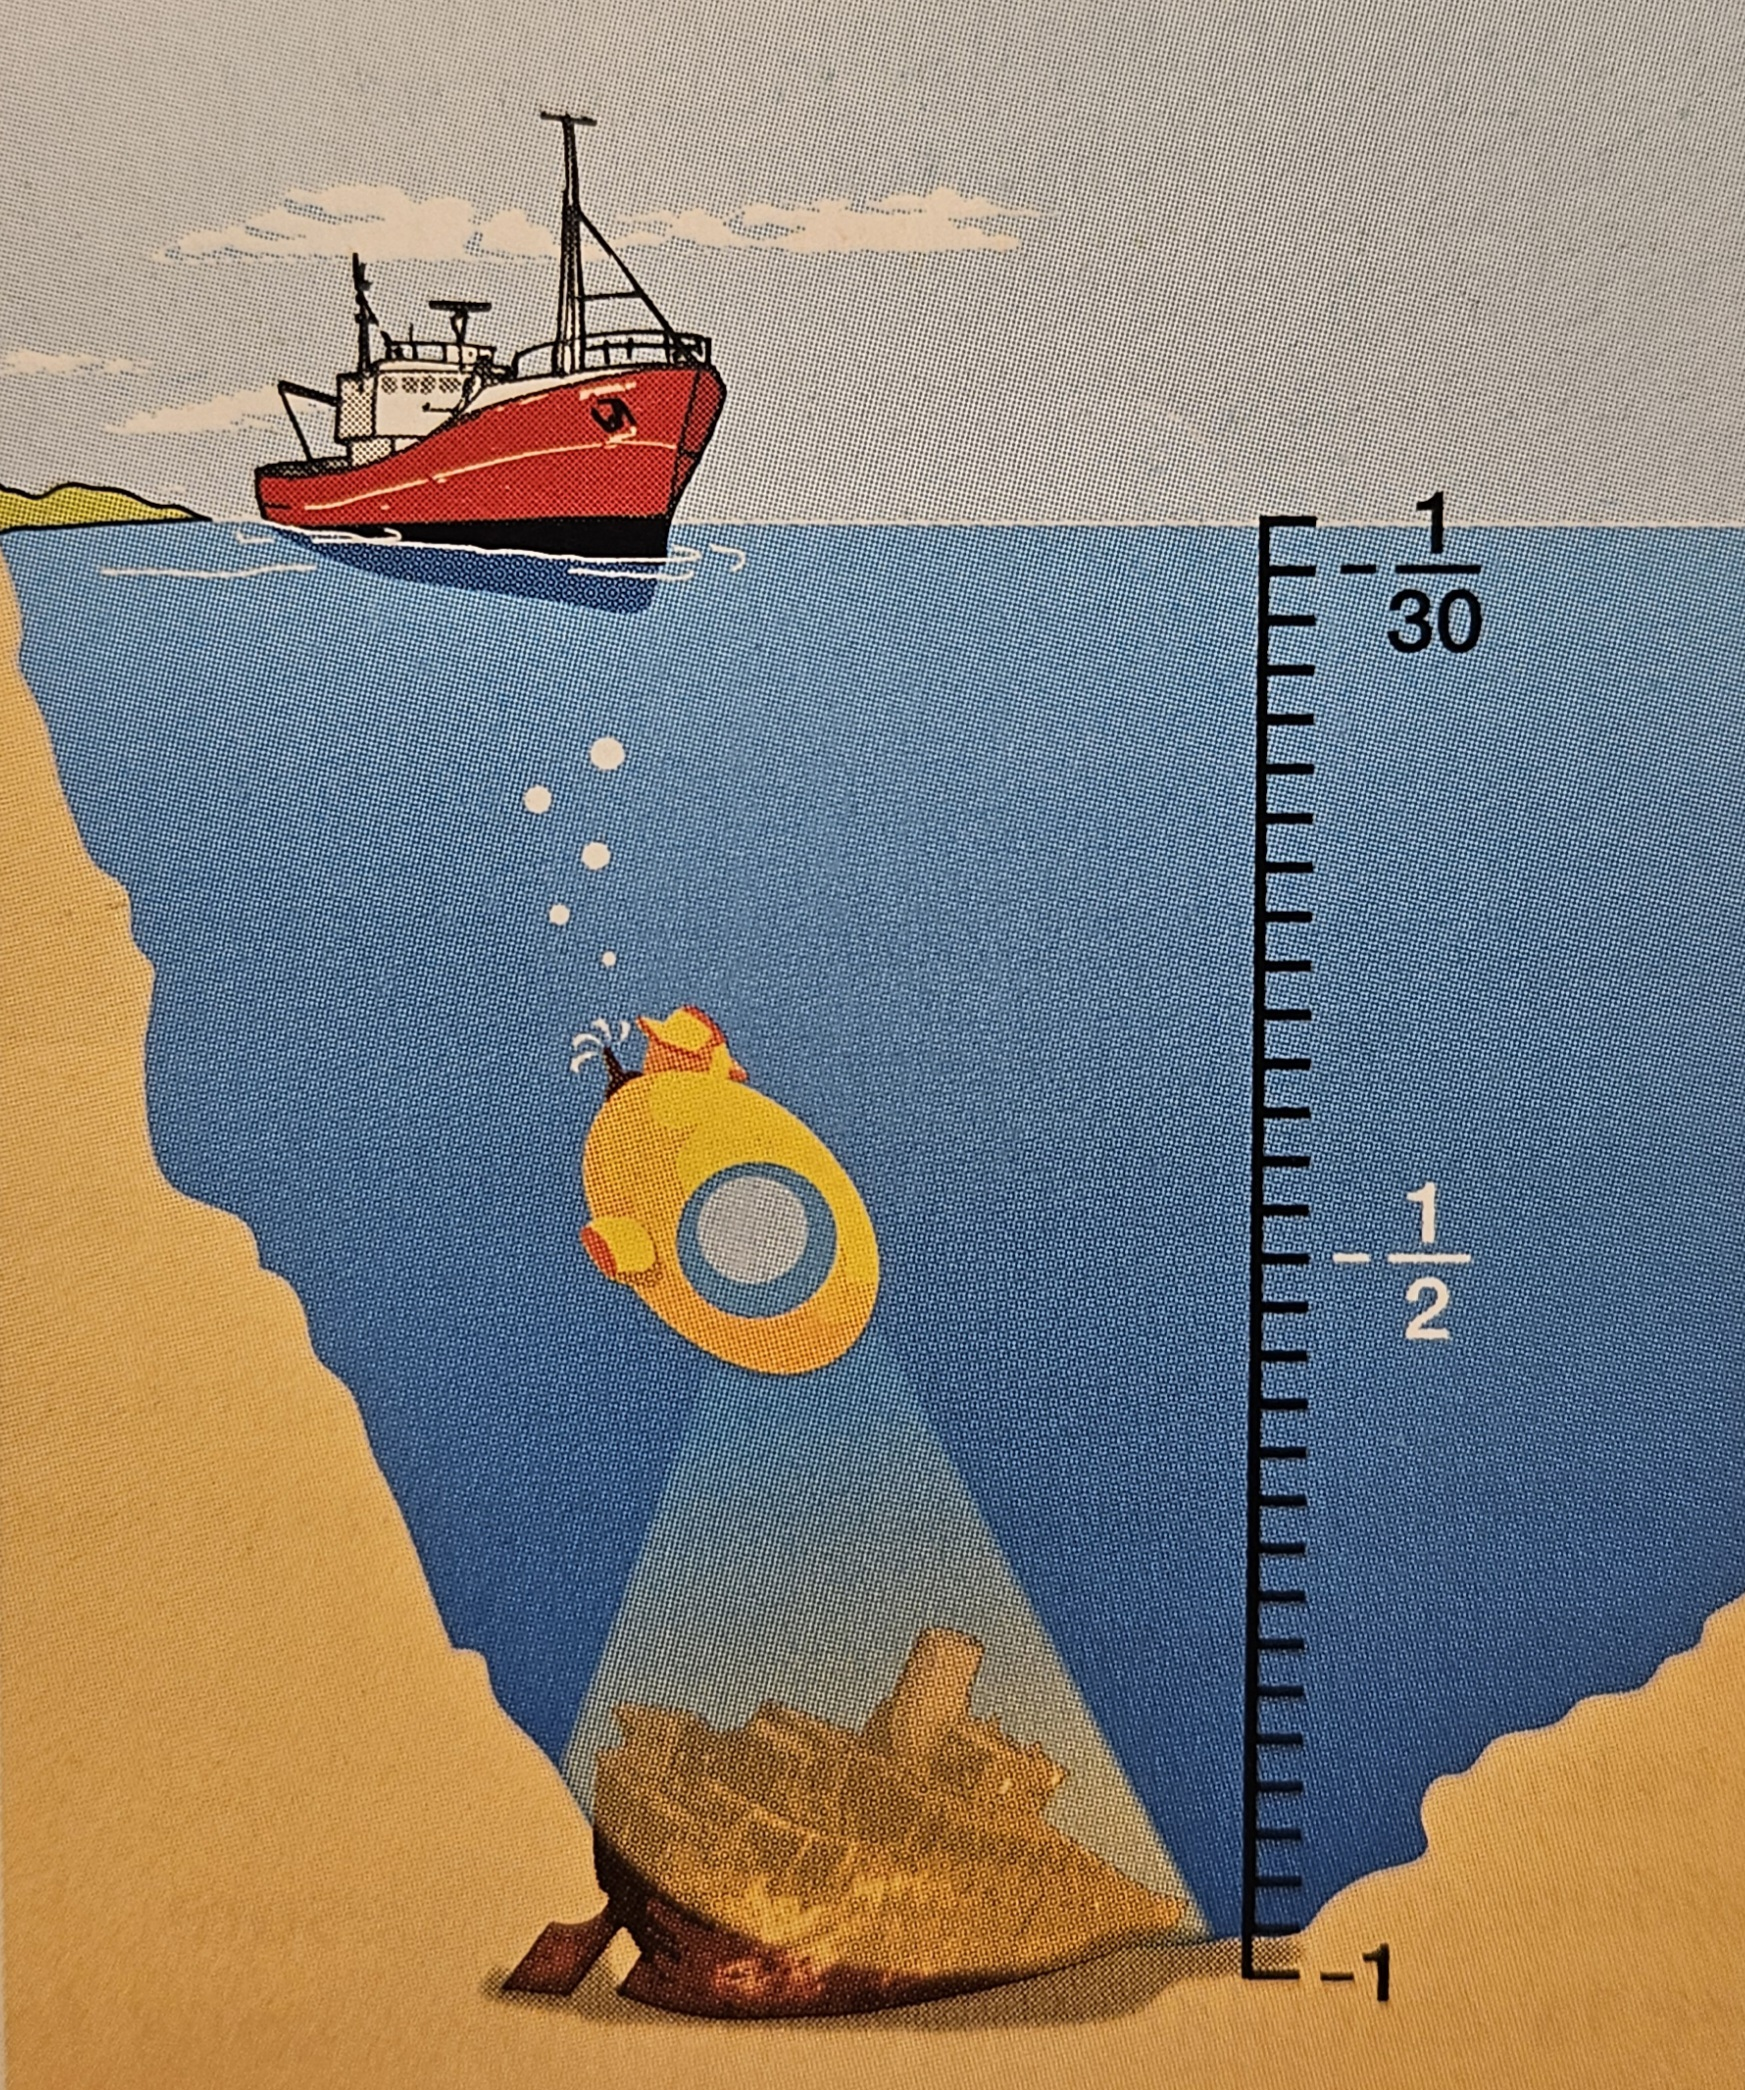
\includegraphics[width=1\textwidth]{exocote.jpg}
\end{minipage}%

\vspace{1cm}

\end{document}
